\chapter{Post-Processing Techniques for Instance Segmentation Masks}\label{ch:postProcessing}

At this stage, the system is capable of detecting cetaceans at an individual pixel level. Before these detections can be passed to the identification module, some post-processing of the output must be performed to allow for both a reduction in the computational expense of operating on the detector's output as well as ensuring that no potentially important information which will assist in an identification is lost. 

\section{Handling Multiple Detections}\label{ch:postProcessing,sec:handlingMultipleDetections}

When an image is ran through the Mask-RCNN detector \cite{he_mask_2017}, the number of outputs can vary depending on how many detected objects have a confidence score higher than 90\% (as discussed in Section \ref{ch:cetDet,sec:ModelSelection,sub:DetectionHyperparameters}). If no detections reach this threshold the image is discarded from further processing. This can occur if, for example, an image is taken by accident capturing the vessel's floor. If a single detection reaches the threshold, the resultant mask is passed downstream. 

Thanks to the tendency for cetaceans to travel in pods however, it is unlikely an image will contain only a single \texttt{dolphin} detection. In these situations the Mask-RCNN will output multiple detection masks, one per object. To handle this, the first stage of the post-processing methodology is to separate multiple detections for a single image. This ensures each \texttt{dolphin} detection is handled independently, mitigating the potential for an identification to be influenced by the others. An example of this behaviour can be seen in Figure \ref{fig:190730-001-MOLS0360_-detections}. Here, an image inputted to the Mask-RCNN detector has produced three detections which are above the threshold. As such, they have been split into three output masks for individual processing. Note that one of the masks, indicated in blue in the Top Left figure, has been incorrectly detected as \texttt{dolphin} with a high confidence. As such a mask has been produced, visualised Bottom Right. Further post-processing must be capable of handling background which has been incorrectly labelled, removing it before individual identification occurs.

\begin{figure}[h]
	\begin{center}
		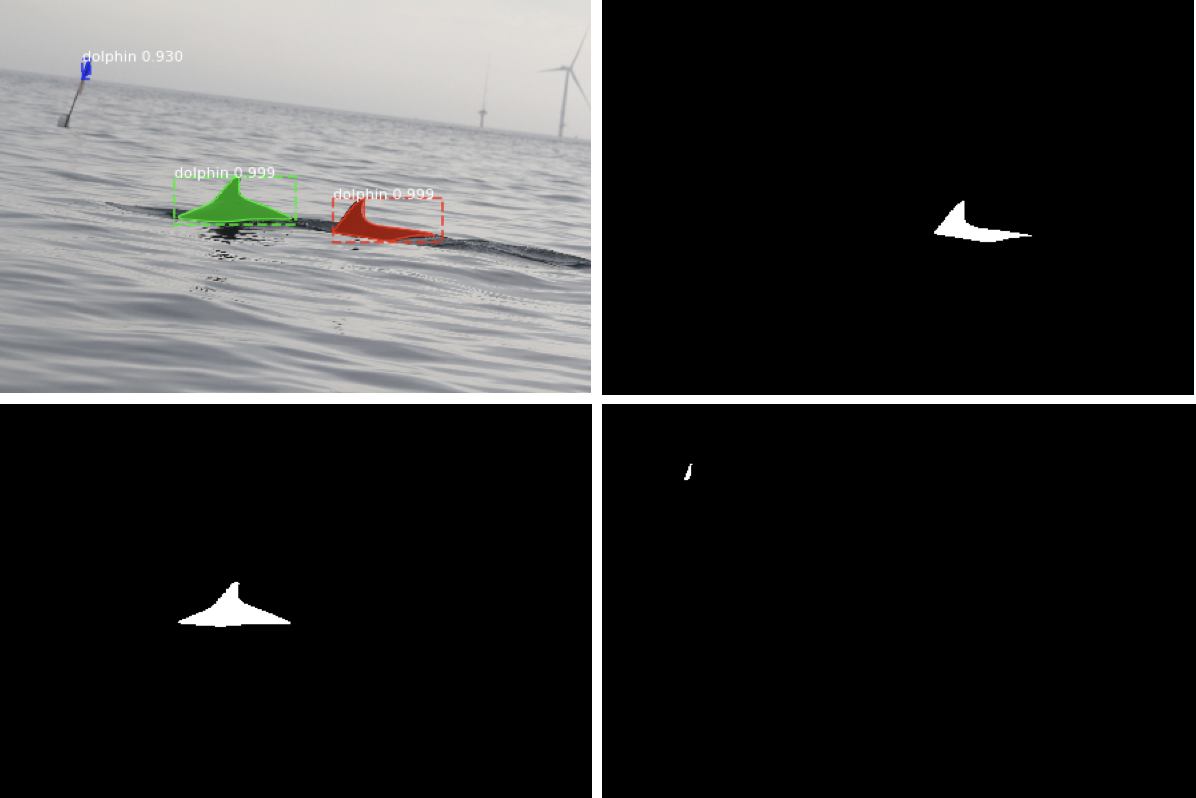
\includegraphics[scale=0.5]{Chapter4/figs/190730-001-MOLS0360_-detections.png}
	\end{center}
	\caption{Top Left: A visualisation of the three \texttt{dolphin} detections for an input image produced by the Mask-RCNN detector, alongside their confidence scores. Top Right, Bottom: The resultant detection masks once split, where \texttt{dolphin} is displayed in white.}
	\label{fig:190730-001-MOLS0360_-detections}
\end{figure}


\section{Morphological Transformations}\label{ch:postProcessing,sec:morphologicalTransformations}

In some situations a detected mask may contain an area of background inside the detection. This can be thought of as a hole in the detection, as seen in Figure \ref{fig:before-and-after-morphing-masks-only} (Left). Using \textit{a priori} knowledge of cetaceans, which would rarely if ever be captured with a hole, it can be deduced that a hole in the detection is highly unlikely and may cause a loss of useful identifying information. As such, any holes which are present in the masks must be filled. This is achieved using morphological transformations, a set of operations which allow for the automated manipulation of the internal structure of binary images such as masks. 

\begin{figure}[h]
	\begin{center}
		
\includegraphics[scale=0.5]{Chapter4/figs/before-and-after-morphing-masks-only.png}
	\end{center}
	\caption{Left: A detection mask before closing has been applied. The detected \texttt{dolphin} object is displayed in white. Note the cluster of black background pixels inside. Right: The same detection mask after closing. Note the pixels which make up the hole have been converted to \texttt{dolphin}.}
	\label{fig:before-and-after-morphing-masks-only}
\end{figure}

The two fundamental morphological transformations are erosion, which erodes away the boundaries of the masked object, and dilation, which increases the size of the object by pushing the boundary out into the background space. These two operations can be utilised in various combinations to perform more complex transformations.

In order to remove a cluster of background pixels inside of a detection, each mask is \textit{closed} - dilated then eroded. This has the effect of removing any holes present inside the mask, as can be seen in Figure \ref{fig:before-and-after-morphing-masks-only} (Right). If no holes exist, the operation is still performed however the mask remains unchanged. By performing closing, the system ensures that no potentially identifiable information is lost as a result of an incomplete detection. 

\section{Background Subtraction}\label{ch:postProcessing,sec:bgExtraction}

Now that the masks have been cleaned using morphological transformations, it is possible to utilise them to perform background subtraction. This is an extremely important step in producing an accurate individual classification based on the detected \texttt{dolphin} object by ensuring a minimal amount of background noise is passed to the identification system.

As both the input image and resultant mask can be represented as matrices, these can be manipulated utilising a \textit{bitwise and} operation such that if pixel$_{i, j}$ in the input image is denoted as background in the mask, the values of pixel$_{i, j}$ can be set to [255, 255, 255] (white). This has the effect of whiting out any pixels not detected as part of the \texttt{dolphin} in the input, whilst keeping the pixels detected as \texttt{dolphin} intact.

An example of background subtraction utilising cleaned masks can be seen in Figure \ref{fig:190730-001-MOLS0360_-bg-subtraction}. Using the same input image as in Figure \ref{fig:190730-001-MOLS0360_-detections}, it can be seen that the \textit{bitwise and} operation whites all pixels in the image except those which have been classified as \texttt{dolphin} for each of the three output masks. Note at this point however that the erroneous classification, shown Bottom Right, still remains. 

\begin{figure}[h]
	\begin{center}
		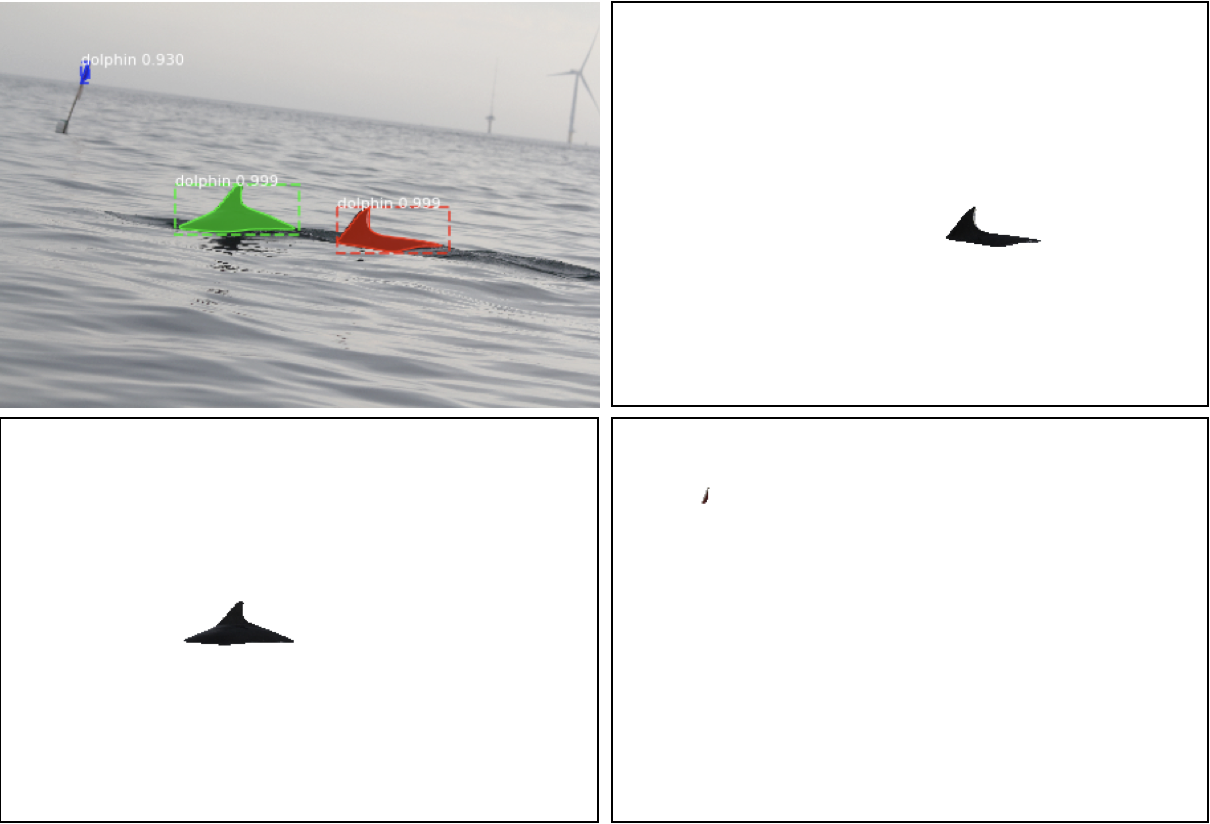
\includegraphics[scale=0.5]{Chapter4/figs/190730-001-MOLS0360_-bg-subtraction.png}
	\end{center}
	\caption{Top Left: A visualisation of the three \texttt{dolphin} detections for an input image produced by the Mask-RCNN detector, alongside their confidence scores. Top Right, Bottom: The resultant output images after \textit{bitwise and} operations performed between the input image and the cleaned detection masks. A border has been added for clarity.}
	\label{fig:190730-001-MOLS0360_-bg-subtraction}
\end{figure}

Whilst the background subtraction aims to reduce noise passed downstream to the individual identification module, it will not be possible to remove all noise. It may be the case, such as in Figure \ref{fig:fin-extraction-unclean}, whereby some background pixels have been mislabelled as \texttt{dolphin} and are connected to those which have been correctly labelled. As a result, morphological transformation and background subtraction are unable to remove the mislabelled pixels. This may affect the accuracy of identification downstream unless the system is robust enough to deal with this.

\begin{figure}
	\begin{center}
		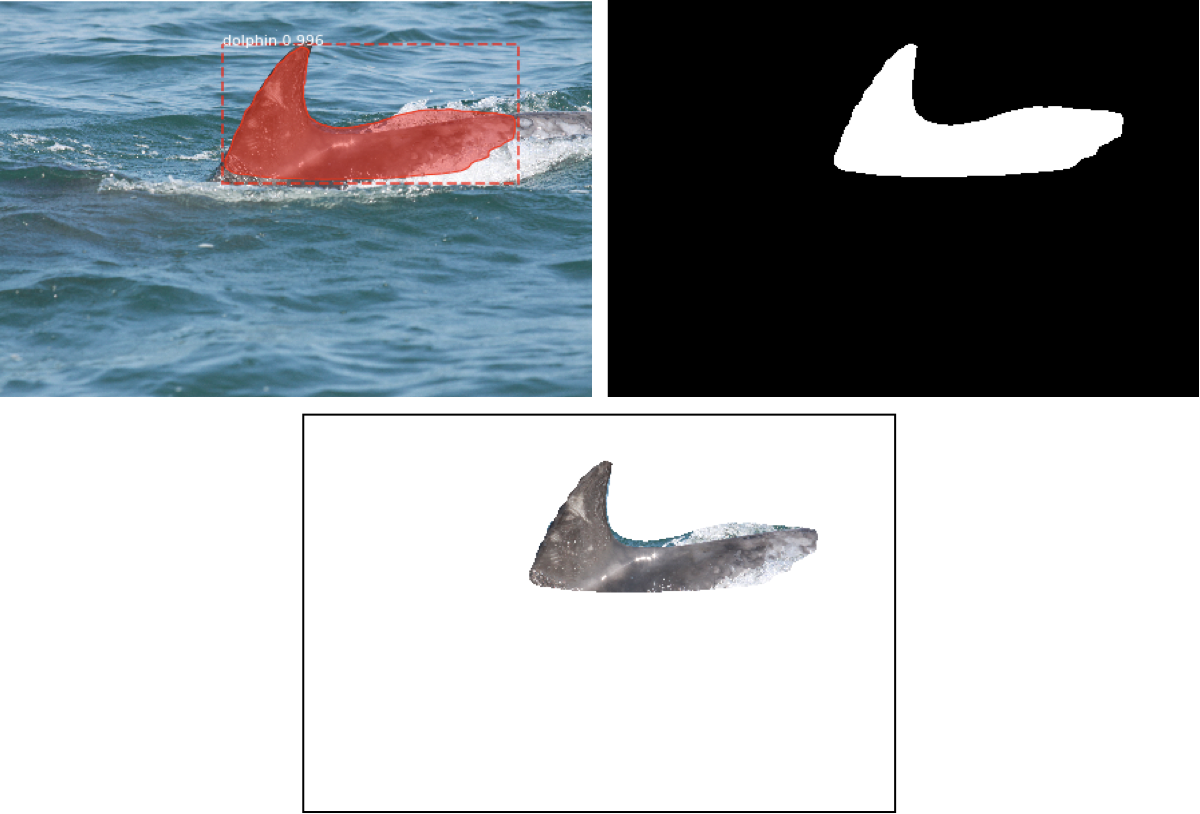
\includegraphics[scale=0.5]{Chapter4/figs/fin-extraction-unclean-uncropped.png}
	\end{center}
	\caption{Top Left: A visualisation of the \texttt{dolphin} detection for an input image produced by the Mask-RCNN detector, alongside the confidence score. The detector has incorrectly labelled some pixels as \texttt{dolphin}. Top Right: The resultant detection mask after morphological transformation. Bottom: The resultant output image after \textit{bitwise and} operations performed between the input image and the cleaned detection mask. Note the mislabelled pixels are present after cleaning and background subtraction. A border has been added for clarity.}
	\label{fig:fin-extraction-unclean}
\end{figure}

\section{Colour Thresholding Mask Components}\label{ch:postProcessing,sec:colourThresholdingMaskComponents}

In some cases a single detection mask may consist of multiple components. This may occur if, for example, an area of disjoint splash has been erroneously included as part of a detection. As cetaceans cannot be made up of multiple disjoint components, it is known that some of these must be noise and can be removed. 

The outer layer of a cetacean's skin is often a consistent grey colouring. This information can be utilised to filter out noisy components of the mask during post-processing. By comparing the colour composition of each detected object against a calculated \textit{dolphin-like} threshold, it is possible to discard mask components which have been erroneously detected.

In order to be able to compare each mask component's composition against a \textit{dolphin-like} colour threshold, the values of the threshold must first be determined. To achieve this, each image in the Zanzibar dataset was ran through the Mask-RCNN detector. Histograms of the three RGB colour channel pixel intensities for each object classification (\texttt{dolphin} or background) were recorded, giving a total of six histograms per image. 

Once complete the histogram groups were combined to give six global pixel intensity distributions, which can be seen in Figure \ref{fig:global-histogram}. From the charts it can be seen that, regardless of colour channel, there is a near inversion in the distribution of pixel intensities between those detected as \texttt{dolphin} and those not, strongly suggesting it is possible to determine if a component is erroneous based on its colour composition.

\begin{figure}
	\begin{center}
		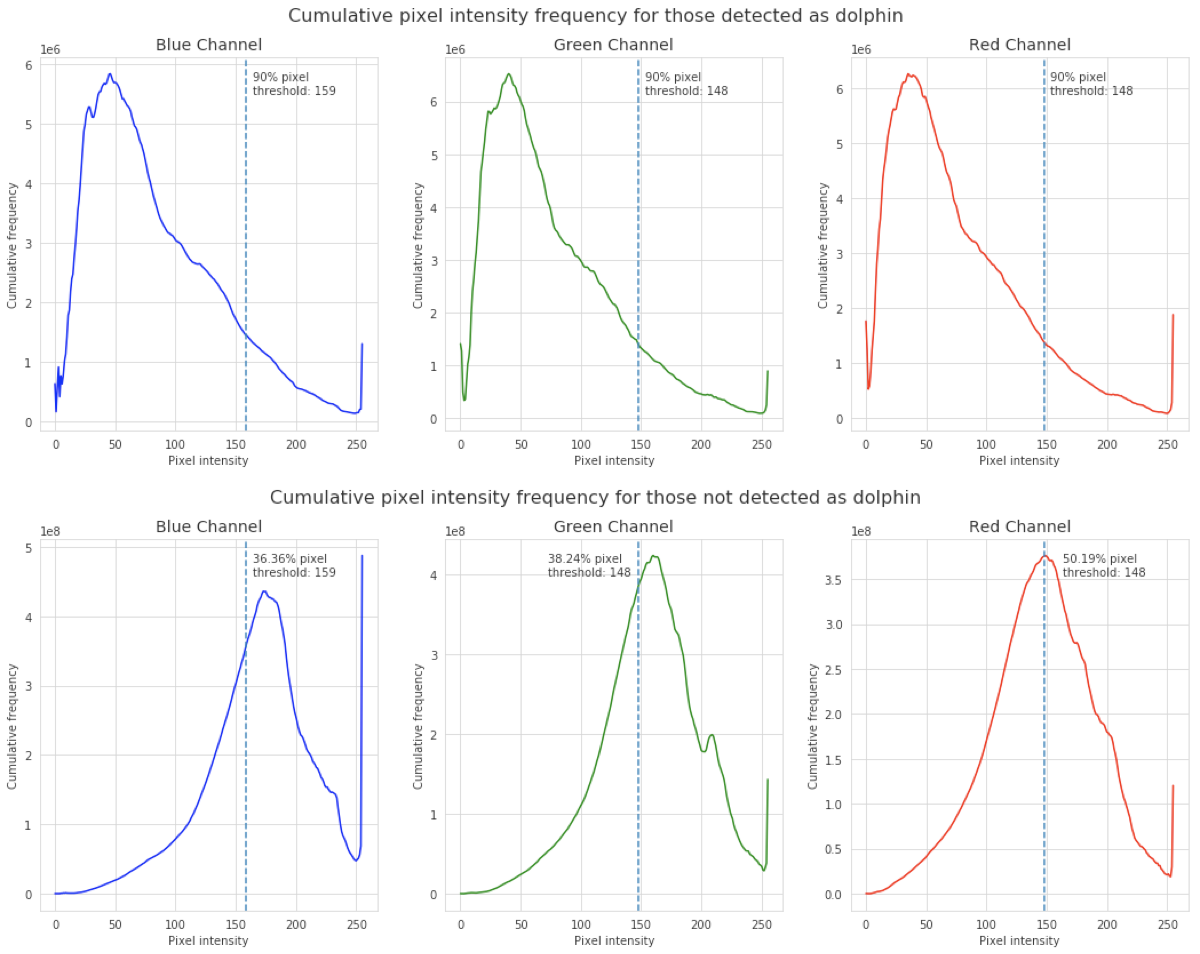
\includegraphics[scale=0.7]{Chapter4/figs/histogram.png}
	\end{center}
	\caption{The global range of pixel intensities for each RGB colour channel, split by pixel classification.}\label{fig:global-histogram}
\end{figure}

Using the global distribution histograms, a \textit{dolphin-like} threshold was determined. For all masks detected as \texttt{dolphin}, 90\% of the RGB pixel intensities are below [148, 148, 159]. The colour representing this threshold can be seen in Figure \ref{fig:colour-threshold}. By contrast only 50.19\%, 38.24\%, and 36.36\% of the background pixels for each RGB channel respectively are below this threshold. As noise components in the mask are often areas of water or splash, these components will be likely much lighter in composition than cetaceans, and thus can be removed from the mask with confidence. An example of colour thresholding removing noise from a mask can be seen in Figure \ref{fig:190827-001-MOLS0078_-colour-thresholding-splash-removed}.
 
 \begin{figure}
 	\begin{center}
 		
\includegraphics[scale=0.3]{Chapter4/figs/148-148-159.png}
 	\end{center}
 	\caption{A representation of the RGB threshold for \textit{dolphin-like}, colour [148, 148, 159]. In the Zanzibar dataset, 90\% of pixels detected as \texttt{dolphin} have intensities below this threshold.}\label{fig:colour-threshold}
 \end{figure}

\begin{figure}
	\begin{center}
		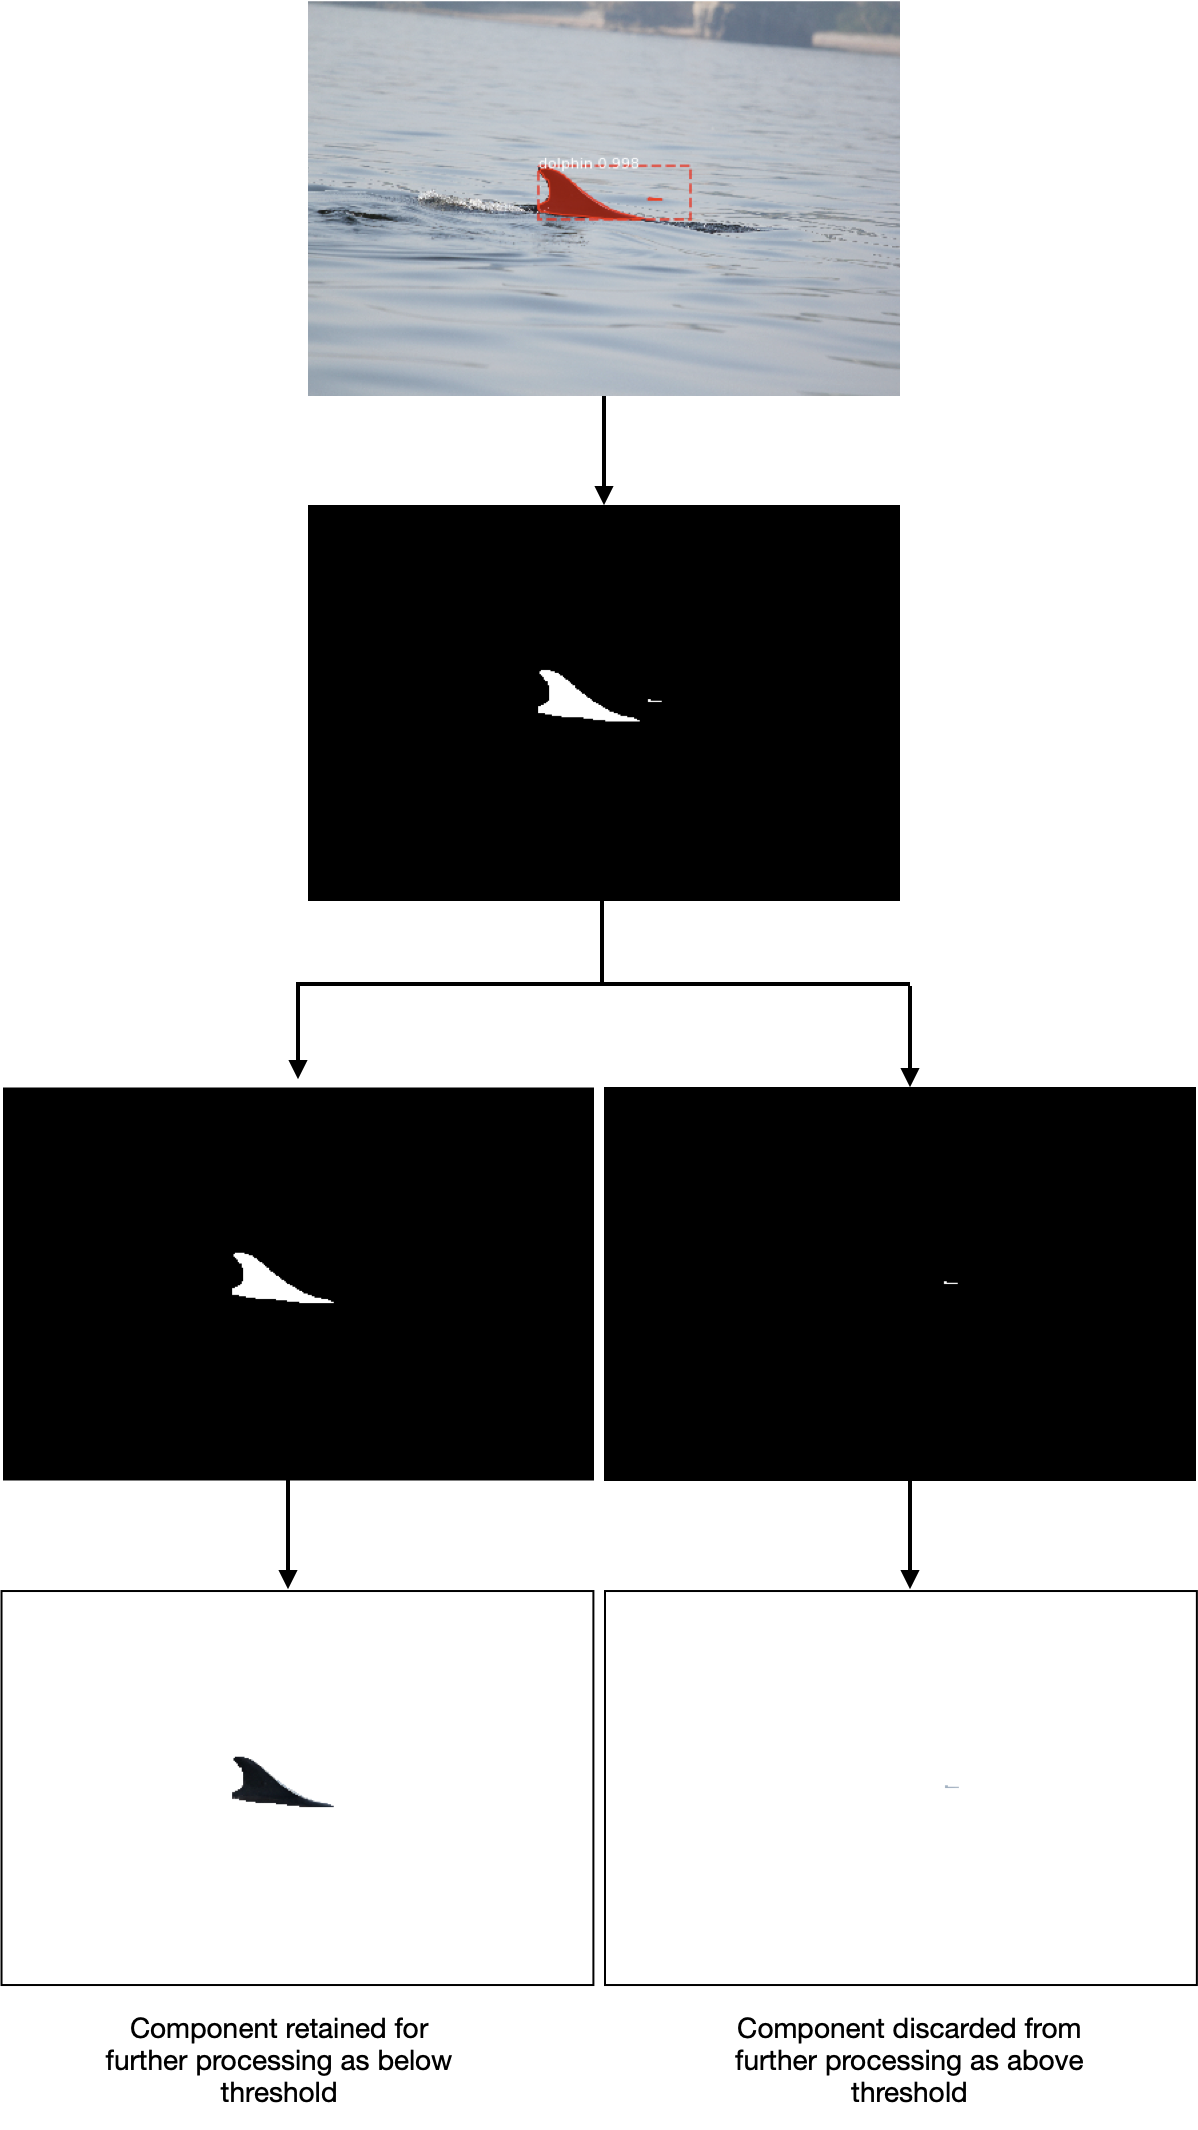
\includegraphics[scale=0.5]{Chapter4/figs/190827-001-MOLS0078_-colour-thresholding-splash-removed.png}
	\end{center}
	\caption{Workflow detailing colour thresholding to remove an area of disjoint splash which has been detected as part of a \texttt{dolphin} object. The detection mask is split into each component. The resultant background subtracted images are then colour thresholded. As a result, the erroneous splash is discarded. }\label{fig:190827-001-MOLS0078_-colour-thresholding-splash-removed}
\end{figure}

During testing however it was found that when checking detections at an individual level rather than globally, considering a mask component to be \textit{dolphin-like} if 90\% of the pixels were below the colour threshold was too restrictive. Utilising such a high percentage bar sometimes rejected valid detections which may have been over-exposed due to lighting conditions. As such, whilst the colour threshold was kept the same, it was found that reducing the percentage check to 50\% provided enough leeway such that over-exposed valid detections were kept whilst still rejecting a large portion of erroneous ones. 

%If multiple components in a mask are below the threshold then keep both as separete masks

It may be the case that multiple components in an image meet the conditions set by the threshold to be kept. In this case, each component of the mask is split into its own image, in a similar process as outlined in Section \ref{ch:postProcessing,sec:handlingMultipleDetections}. If a mask only contains one component, then colour thresholding is not applied. This ensures no detections by the Mask-RCNN are completely ignored due to post-processing, preventing the discarding of a \texttt{dolphin} object mask which contains no disjoint components however is above the threshold, such as in the event of over-exposure. This condition has the effect of allowing fully erroneous detections to pass downstream, such as the flag detected in Figures \ref{fig:190730-001-MOLS0360_-detections} and \ref{fig:fin-extraction-unclean}. Any erroneous detections which pass downstream at this stage must now be handled by the identification module.

\section{Cropping}\label{ch:postProcessing,sec:cropping}

At this point outputs from the Mask-RCNN detector have been post-processed to remove as many erroneous detections as possible, and these have been utilised to perform background subtraction. This results in an output image containing mostly white pixels surrounding a detected \texttt{dolphin} object. This image is the same size as the one inputted to the detector, which can often be many thousands of pixels, although the vast majority of these are now un-needed.

%TODO: Add figure showing cropping, get image sizes before and after.

As a result, the image outputted from the background detector are now cropped down to contain just the object of interest. This has the effect of vastly reducing the image file size, which in turn reduces the computational expense of operating on them downstream. In Figure XXX for example, the input image to the detector is of size YYY. After post-processing, the resulting output image is now of size ZZZ, a LLLx reduction. This cropping also has the effect of centring the detected \texttt{dolphin} objects in the image. 


%=================
%
%\section{Background Subtraction \& Cropping}\label{ch:postProcessing,sec:bgExtraction}
%
%One of the main components of the post-processing pipeline is the background subtraction module. 
%
%As both the input image and its resultant mask can be represented as matrices, these can be manipulated utilising a \textit{bitwise and} operation such that if pixel$_{i, j}$ in the input image is denoted as background in the mask, the values of pixel$_{i, j}$ can be set to [255, 255, 255] (white). This has the effect of whiting out any pixels not detected as part of the fin in the image, removing noise. 
%
%Once the background subtraction has been achieved the input image can then be cropped to reduce file size. By using the top, bottom, left, and right-most non-white pixels in the image as bounding box coordinates for the fin, the input image can be vastly reduced, often to only a few hundred pixels in both height and width. This greatly reduces the computational expense of further operations downstream by reducing the size of subsequent input images passed to other components. 
%
%Figure \ref{fig:fin-extraction-clean} shows the effect of performing background subtraction on an input image, with the detected \texttt{dolphin} pixels from the Mask-RCNN highlighted in red. As can be seen, the background subtraction and cropping has resulted in a clean image of the animal's dorsal fin. Identifying information is present, with minimal levels of noise. 
%
%\begin{figure}[h]
%	\begin{center}
%		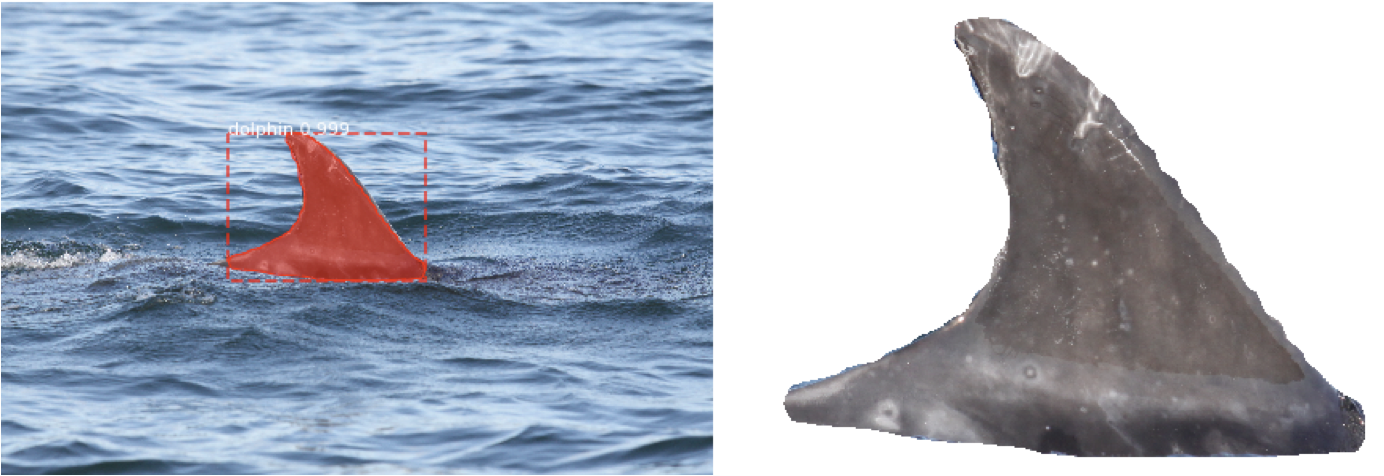
\includegraphics[scale=0.5]{Chapter4/figs/fin-extraction-clean.png}
%	\end{center}
%	\caption{The effect of background subtraction and cropping on an input image, left. The detected \texttt{dolphin} pixels by the Mask-RCNN have been highlighted in red with confidence score shown. The resultant output, right, has been enlarged for visibility.}
%	\label{fig:fin-extraction-clean}
%\end{figure}
%
%Whilst the background subtraction module aims to reduce as much noise as possible entering the identification module, which can be achieved thanks to the high accuracy of the detector, it will not be possible to remove all noise. It may be the case, such as in Figure \ref{fig:fin-extraction-unclean}, whereby some background has been mislabelled as \texttt{dolphin}. As a result, the background subtraction module is unable to remove the mislabelled background pixels which may effect the accuracy of the identification downstream unless the system is robust enough to deal with this.
%
%\begin{figure}[h]
%	\begin{center}
%		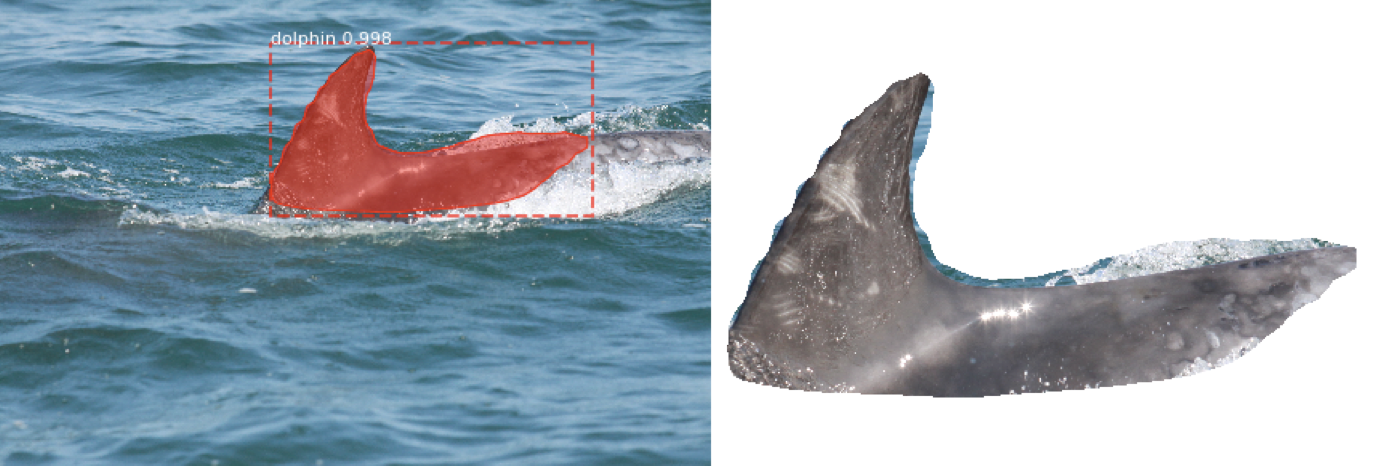
\includegraphics[scale=0.5]{Chapter4/figs/fin-extraction-unclean.png}
%	\end{center}
%	\caption{The result of background subtraction and cropping where the detector has mislabelled some background pixels as \texttt{dolphin}, right. Detected pixels have been highlighted red on the input image, left, with confidence score shown.}
%	\label{fig:fin-extraction-unclean}
%\end{figure}
%
%As cetaceans often travel in pods containing multiple individuals, any post-processing methodology must be capable of handling this. To account for this, if the background subtraction module is passed multiple masks for an image it operates on each mask independently. This results in potentially multiple output images per input, one for each detection. An example of this behaviour can be seen in Figure \ref{fig:fin-extraction-pod-with-flag}.
%
%\begin{figure}[h]
%	\begin{center}
%		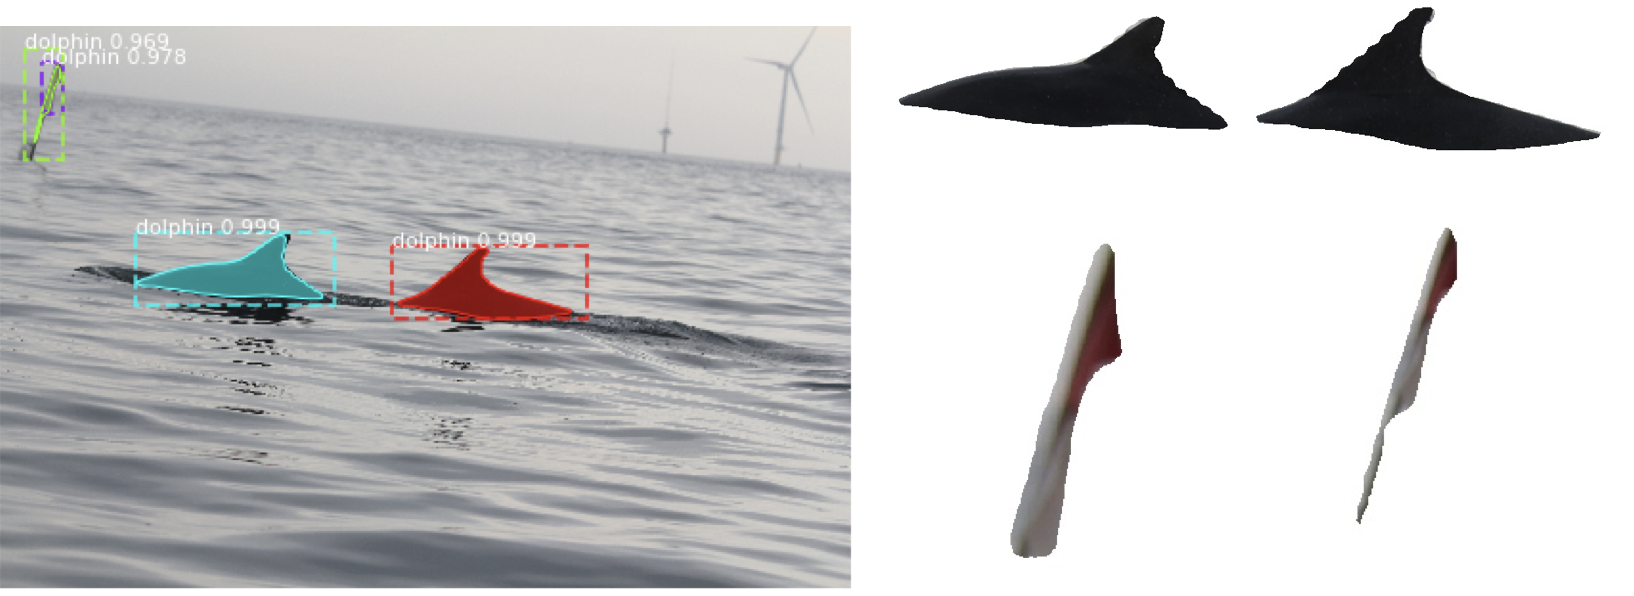
\includegraphics[scale=0.5]{Chapter4/figs/fin-extraction-pod-with-flag.png}
%	\end{center}
%	\caption{The result of background subtraction and cropping where the detector is passed multiple masks for an input image, right. Detections and confidence scores are overlaid onto the input image, left.}
%	\label{fig:fin-extraction-pod-with-flag}
%\end{figure}
%
%As the Mask-RCNN has detected four \texttt{dolphin} objects in the image, the background subtraction and cropping module has produced four output images. However it can be seen that two of the detections have been misclassified - they are actually of a flag denoting the location of a lobster pot and thus should be background. Further post-processing of the detection outputs is required to ensure the minimal amount of erroneous detections are passed downstream without stopping correct classifications. 
%
%
%
%% Rejig this chapter to follow format in Log 16/3


%%%%%%%%%%%%%%%%%%%
\nomenclature[z-CNN]{CNN}{Convolutional Neural Networks}

